%!TEX root = ../Thesis.tex
%Chapter 1

\chapter{Asymmetric scattering by non-Hermitian potentials}
\label{Chapter1}
\lhead{Chapter 1. \emph{Asymmetric scattering by non-Hermitian potentials}}
%
The scattering of quantum particles by non-hermitian (generally nonlocal)  potentials in one dimension
may result in asymmetric transmission and/or reflection from left and right incidence.
After extending the concept of symmetry for nonhermitian potentials, eight generalized symmetries based on the discrete  Klein's four-group
(formed by parity, time reversal, their product, and unity) are found. Together with generalized unitarity relations they determine
selection rules for the possible and/or forbidden scattering asymmetries.
Six basic device types are
identified when the scattering coefficients (squared moduli of scattering amplitudes)
adopt zero/one values, and transmission and/or reflection are asymmetric.
They can pictorically be described as a
one-way mirror, a one-way barrier (a Maxwell  pressure demon), one-way (transmission or reflection) filters,
a mirror with unidirectional transmission, and a transparent, one-way reflector. We design potentials
for these devices and also demonstrate that the  behavior of the scattering
coefficients can be extended to a broad range of incident momenta.
%
\newpage
%
\section{Introduction}

The current interest to develop new quantum technologies is boosting applied and fundamental
research on quantum phenomena and on systems with potential applications in logic circuits, metrology, communications or sensors.
Robust basic devices performing elementary operations are needed to perform
complex tasks when combined in a circuit.

In this paper we investigate the properties of potentials with asymmetric
transmission or reflection for a quantum, spinless particle of mass $m$ satisfying a one-dimensional (1D) Schr\"odinger equation. If we restrict the analysis  to  transmission and reflection coefficients (squared moduli
of the scattering complex amplitudes) being  either zero or one, a useful simplification for quantum logic operations,
there are six types of asymmetric devices, see fig. \ref{cases}.
These devices cannot be constructed with Hermitian potentials. In fact for all device types with transmission asymmetries,
which are four of the six possible devices,
the potentials have to be also nonlocal. Therefore, nonlocal potentials play a major role in this paper. They appear naturally when applying partitioning techniques
under similar conditions to the
ones leading to non-hermitian  potentials, namely, as effective interactions for a subsystem or component of the full wave-function,
even if the interactions for the large system are hermitian and local \cite{Muga2004}.

Symmetries can be used, similarly to their standard application in atomic physics to determine selection rules for allowed/forbidden
transitions,
to predict whether a certain potential may or may not lead to asymmetric
scattering. The concept of symmetry, however, must be generalized when dealing with non-hermitian potentials.

The theory in this paper is worked out for particles and the Schr\"odinger equation but it is clearly of relevance for optical devices
due to the much exploited analogies and connections between Maxwell's equations and the Schr\"odinger equation,
which were used, e.g., to propose  the realization of PT-symmetric potentials in optics \cite{Ruschhaupt2005}.


\begin{figure}
  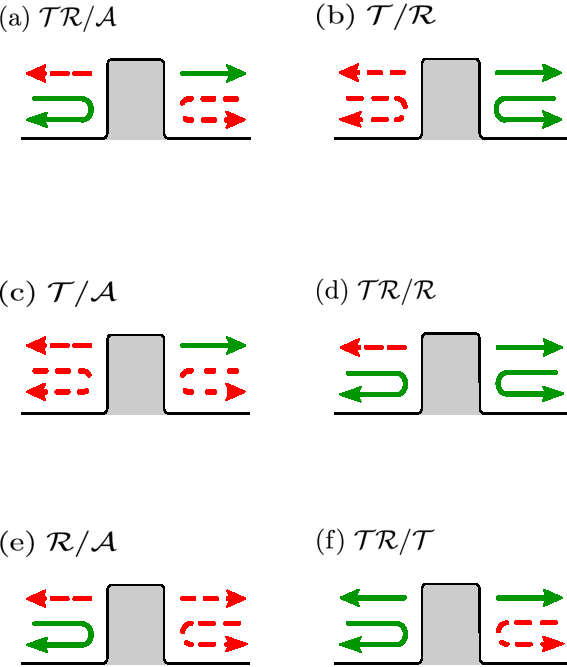
\includegraphics[width = 0.9\columnwidth]{Figures/PotentialCasesPT.pdf}
  \caption{(Color online) Devices with asymmetric scattering (limited to scattering coefficients being 0 or 1).  The dashed and continuous lines represent respectively zero or one
  for the moduli of the scattering amplitudes; the bended lines are for reflection amplitudes, and the straight lines for transmission:
  (a) One-way mirror ($\cal{TR/A}$); (b) One-way barrier ($\cal{T/R}$); (c) One-Way T-filter ($\cal{T/A}$);
  (d) Mirror \& 1-way transmitter ($\cal{TR/R}$); (e) One-way R-filter ($\cal{R/A}$); (f) Transparent, one-way
  reflector ($\cal{TR/T}$).
  The letter codes summarize the effect of left and right incidence, separated by a  slash ``$/$''.
  ${\cal T}$ or ${\cal R}$ on one side of the slash indicate a unit
  transmission or reflection coefficient
  for  incidence from that side, whereas the absence of one or the other letter corresponds to zero coefficients.
  An ${\cal A}$ denotes ``full absorption'', i.e., both moduli of reflection and transmission amplitudes are zero for incidence from one side.
  For example,  $\cal{TR/A}$ means unit modulus transmission
  and reflection from the left and total absorption from the right.
  \label{cases}}
\end{figure}


% ----------------------------------------------------------------------------------------------
\begin{landscape}
  \begin{table}
    \caption{Symmetries of the potential classified in terms of the commutativity or pseudo-hermiticity of $H$ with the elements of
    Klein's 4-group  $\{1,\Pi,\theta,\Pi\theta\}$ (second column). The first column sets a simplifying roman-number code for each symmetry.
    The relations among potential matrix elements are given in coordinate and momentum representations in the third and fourth columns.
    The fifth column gives the relations they imply in the matrix elements of $S$ and/or $\widehat{S}$ matrices ($S$ is for scattering by $H$
    and $\widehat{S}$ for scattering by $H^\dagger$). From them  the next four columns set the relations implied on scattering amplitudes.
    Together with generalized unitarity relations (\ref{gur}) they also imply relations for the moduli (tenth column), and phases (not shown). The last two columns indicate the possibility to achieve perfect asymmetric transmission or reflection:  ``${P}$" means possible (but not necessary),
    ``No'' means impossible.  In some cases ``$P$" is accompanied by a condition that must be satisfied.\vspace*{.2cm}
    \label{table2}}
    \centering
    \scalebox{0.75}{
    \begin{tabular}{cccccccccccc}
      %\hline
      Code & Symmetry&  $\langle x|V|y\rangle=$ & $\langle p|V|p'\rangle=$ & $\langle p|S|p'\rangle=$ & $T^l\!=$ & $T^r\!=$ & $R^l\!=$& $R^r\!=$& from eq. (\ref{gur})&$|T^l|\!=\!1$&$|R^l|\!=\!1$
      \\
      &&&&&&&&&&$|T^r|\!=\!0$&$|R^r|\!=\!0$
      \\
      \hline
      I & $1H=H1$ &   $\langle x|V|y\rangle$ & $\langle p|V|p'\rangle$ & $\langle p|S|p'\rangle$ & $T^l$ & $T^r$ & $R^l$ & $R^r$ & & $P$ & $P$
      \\
      II & $1H=H^\dagger 1$ &  $\langle y|V|x\rangle^*$ & $\langle p'|V|p\rangle^*$ &$\langle p|\widehat{S}|p'\rangle$ & $\widehat{T}^l$& $\widehat{T}^r$ & $\widehat{R}^l$ & $\widehat{R}^r$
      & $|T^l|\!=\!|T^r|$, $|R^l|\!=\!|R^r|$&No&No
      \\
      III & $\Pi H=H\Pi$ &  $\langle -x|V|-y\rangle$ & $\langle -p|V|-p'\rangle$ &$\langle -p|S|-p'\rangle$ & $T^r$ & $T^l$ & $R^r$ & $R^l$& $|T^l|\!=\!|T^r|$,$ |R^l|\!=\!|R^r|$ &No&No
      \\
      IV & $\Pi H=H^\dagger \Pi$ &  $\langle -y|V|-x\rangle^*$ & $\langle -p'|V|-p\rangle^*$ & $\langle -p|\widehat{S}|-p'\rangle$ & $\widehat{T}^r$ & $\widehat{T}^l$ & $\widehat{R}^r$ & $\widehat{R}^l$&&$P$, $R^rR^{l*}=1$&$P$, $T^r{T^l}^*=1$
      \\
      V & $\Theta H=H\Theta$ &  $\langle x|V|y\rangle^*$& $\langle -p|V|-p'\rangle^*$ & $\langle -p'|\widehat{S}|-p\rangle$ & $\widehat{T}^r$ & $\widehat{T}^l$ & $\widehat{R}^l$& $\widehat{R}^r$
      &$|R^l|=|R^r|$&$P$, $|R^{r,l}|=1$&No
      \\
      VI & $\Theta H=H^\dagger\Theta$ &  $\langle y|V|x\rangle$& $\langle -p'|V|-p\rangle$ & $\langle -p'|S|-p\rangle$ & $T^r$& $T^l$ & $R^l$& $R^r$&$|T^l| = |T^r|$&No&$P$
      \\
      VII & $\Theta\Pi H=H\Theta \Pi$ &  $\langle -x|V|-y\rangle^*$ & $\langle p|V|p'\rangle^*$ & $\langle p'|\widehat{S}|p\rangle$ &$\widehat{T}^l$& $\widehat{T}^r$ & $\widehat{R}^r$& $\widehat{R}^l$&$|T^l|=|T^r|$&No&$P$, $|T^{r,l}|=1$
      \\
      VIII& $\Theta\Pi H=H^\dagger \Theta \Pi$ &  $\langle -y|V|-x\rangle$ & $\langle p'|V|p\rangle$ & $\langle p'|S|p\rangle$ & $T^l$ & $T^r$ & $R^r$ & $R^l$&$|R^l|=|R^r|$&$P$&No
      %\\
      %\hline
    \end{tabular}}
  \end{table}
\end{landscape}

% ----------------------------------------------------------------------------------------------




\section{Generalized symmetries}


The detailed technical and formal background for the following can be found in
a previous review on 1D scattering by complex potentials \cite{Muga2004}, a companion to this article
for those readers willing to reproduce the calculations in detail.
The Supplemental Material (Sec. I)  provides also a minimal kit of scattering theory formulae that may be
read first to set basic concepts and notation.
The notation is essentially as in \cite{Muga2004}, but it proves convenient to use
for the potential matrix (or kernel function) in coordinate representation
two different forms, namely $\langle x|V|y\rangle=V(x,y)$. ``Local'' potentials are those
for which $V(x,y)=V(x)\delta(x-y)$.



%
For hermitian  Hamiltonians, symmetries are represented by the commutation of
a symmetry operator with the Hamiltonian. In scattering theory, symmetry plays an important role  as it implies relations among
the S-matrix elements beyond those implied by its unitarity, see e.g. \cite{Taylor1972} and, for scattering in one dimension,
Sec. 2.6 in \cite{Muga2004}.

Symmetries are also useful for  non-hermitian Hamiltonians, but the mathematical and conceptual
framework must be generalized. We consider that a unitary or antiunitary operator $A$ represents a symmetry of $H$ if it satisfies
at least one of these relations,
%
\begin{eqnarray}
  AH&=&HA,
  \label{symm}
  \\
  AH&=&H^\dagger A.
  \label{pseudo}
\end{eqnarray}
%
For a right eigenstate of $H$, $|\psi\rangle$,
with eigenvalue $E$, eq. (\ref{symm}) implies that
$A|\psi\rangle$ is also a right  eigenstate of $H$, with the
same eigenvalue if $A$ is unitary, and with the complex conjugate eigenvalue $E^*$ if $A$ is antiunitary.
Equation (\ref{pseudo}) implies that $A|\psi\rangle$ is a right eigenstate of $H^\dagger$
with eigenvalue $E$ for $A$ unitary or $E^*$ for $A$ antiunitary, or a left eigenstate of $H$ with eigenvalue $E^*$ for $A$ unitary, or $E$
for $A$ antiunitary. For real-energy scattering
eigenfunctions in the continuum, the ones we are interested in here, $E^*=E$.
When eq. (\ref{pseudo}) holds we say that $H$ is $A$-pseudohermitian \cite{Mostafazadeh2010}.
Parity-pseudohermiticity has played an important role as being equivalent to space-time reflection (PT) symmetry for {\it local} potentials
\cite{Mostafazadeh2010,Znojil2015}. A large set of these equivalences
will be discussed below.
A relation of the form (\ref{pseudo}) has been also used with differential operators  to get real spectra beyond
PT-symmetry for local potentials  \cite{Nixon2016,Nixon2016a}.

Here we consider
%that $H$ may be non-local, and
$A$ to be a member of the
Klein 4-group $K_4=\{1,\Pi, \Theta, \Pi\Theta\}$ formed by unity, the parity operator $\Pi$, the antiunitary time-reversal operator $\Theta$, and their product
$\Pi\Theta$. This is a discrete, abelian group.
We also assume that the  Hamiltonian is  of the form $H=H_0+V$, with $H_0$, the kinetic energy operator of the particle,
being hermitian and
satisfying $[H_0,A]=0$ for all members of the group, whereas the potential $V$ may be non-local in position representation.
The  motivation to use Klein's group is that the eight relations implied by eqs. (\ref{symm}) and (\ref{pseudo}) generate all
possible symmetries of a non-local potential due to the identity, complex conjugation, transposition, and sign inversion,
both in coordinate or momentum representation, see table \ref{table2}, where each symmetry has been labeled by a roman number.
Interesting enough, in this classification hermiticity (symmetry II in  table \ref{table2})
may be regarded as $1$-pseudohermiticity.

\begin{table}
  \caption{Equivalences among symmetries for the potential elements.
  Given the symmetry of the upper row, the table provides the equivalent symmetries.
  For example, if II is satisfied, then III=IV holds. In words, if the potential is hermitian,  parity symmetry amounts to
  parity pseudohermiticity. In terms of the matrix elements of the potential, if  $\langle x|V|y\rangle=\langle y|V|x\rangle^*$ {\it and also}
  $\langle x|V|y\rangle=\langle -x|V|-y\rangle$, $\forall (x,y)$, then $\langle x|V|y\rangle=\langle -y|V|-x\rangle^*$ holds as well. One may proceed similarly for all other relations.
  The commutation with the identity (I) is excluded as this symmetry is satisfied by all potentials.\vspace*{.2cm}
  \label{tablee}}
  \centering
  \scalebox{0.9}{
  \begin{tabular}{ccccccc}
    %\hline
    II & III& IV& V& VI & VII &VIII
    \\
    \hline
    III=IV & II=IV & II=III & II=VI &II=V&II=VIII&II=VII
    \\
    V=VI&V=VII&V=VIII&III=VII&III=VIII&III=V&III=VI
    \\
    VII=VIII&VI=VIII&VI=VII&IV=VIII&IV=VII&IV=VI&IV=V
    %\\
    %\hline
  \end{tabular}}

\end{table}

Examples on how to find the relations in the fifth column of table \ref{table2} of $S-$ and $\widehat{S}$-matrix elements (for scattering by $H$ and $H^\dagger$ respectively)
are provided in
ref. \cite{Muga2004}, where the symmetry types III, VI, and VII where worked out. Similar manipulations, making use of the action of unitary or antiunitary operators
of Klein's group on M\"oller operators, help to
complete the  table.

From the fifth column in table 1, equivalences among the amplitudes for left and right incidence
for scattering by $H$, ($T^{l,r}, R^{l,r}$) or $H^\dagger$  ($\widehat{T}^{l,r}, \widehat{R}^{l,r}$),
are deduced, see the Supplemental Material  and the four columns for
$T^{l,r}$, and $R^{l,r}$ in table \ref{table2}.
Together with the generalized unitarity relations $\widehat{S}^\dagger S=S\widehat{S}^\dagger=1$,
which in terms of amplitudes take the form \cite{Muga2004}
%(\ref{gur}),
%
\begin{eqnarray}
  \widehat T^l T^{l*} + \widehat R^l R^{l*} = 1,
  \nonumber\\
  \widehat T^r T^{r*} + \widehat R^r R^{r*} = 1,
  \nonumber\\
  \hat T^{l*} R^r + T^r \widehat R^{l*} = 0,
  \nonumber\\
  T^l \widehat R^{r*} + \widehat T^{r*} R^l = 0,
  \label{gur}
\end{eqnarray}
%
these equivalences  between the amplitudes
imply further consequences on the amplitudes' moduli (tenth column of table \ref{table2}) and phases (not shown).
The final two columns use the previous results to determine if perfect asymmetry is possible for transmission or reflection.
This makes evident that hermiticity (II) and parity (III) preclude, independently, any asymmetry in the scattering coefficients;
PT-symmetry (VII) or  $\Theta$-pseudohermiticity
(VI) forbid transmission asymmetry (all local potentials  satisfy automatically
symmetry VI),  whereas time-reversal symmetry (i.e., a real potential in coordinate space)
(V) or  PT-pseudohermiticity (VIII) forbid reflection asymmetry.
A caveat is that asymmetric effects forbidden by a certain symmetry in the linear (Schr\"odinger)
regime considered in this paper might not be forbidden in a non-linear regime \cite{Xu2014}, which goes beyond our present scope.

The occurrence of one particular symmetry in the potential (conventionally  ``first symmetry'')
does not exclude a second symmetry to be satisfied as well.
When a double symmetry holds, excluding the identity,  the ``first'' symmetry  implies the equivalence of the second symmetry with a third symmetry.
We have already mentioned that $\Pi$-pseudohermiticity (IV) is equivalent to $PT$-symmetry (VII) for local potentials.
Being local is just one particular way to satisfy symmetry VI, namely $\Theta$-pseudohermiticity. The reader may verify with the aid of
the third column for $\langle x|V|y\rangle$  in table \ref{table2}, that indeed, if symmetry VI is satisfied (first symmetry), symmetry IV has the same effect as symmetry VII.
They become equivalent. Other well known example is  that for a local potential (symmetry VI is satisfied), a real potential in coordinate space  is necessarily hermitian,
so symmetries V and II become equivalent.
These examples are just particular cases of the full set of equivalences given in table \ref{tablee}.

\begin{landscape}
  \begin{table}
    \caption{Device types for  transmission and/or reflection asymmetry, restricted to 1 or 0 moduli for the scattering amplitudes.
    % (i.e., zero scattering amplitudes for transmission and reflection from the right).
    The fifth column indicates the symmetries in table \ref{table2} that forbid the device. Figures S2, S3, S5 and S6 can be found in the supplemental material to this paper.\vspace*{.2cm}}
    \label{table1}
    \centering
    \scalebox{0.85}{
    \begin{tabular}{ccccccc}
      %\hline
      Device type & Left incidence& Right incidence&Code& Forbidden by & Example
      \\
      \hline
      One-way mirror&transmits and reflects&absorbs&$\cal{TR/A}$&II, III, IV, V, VI,  VII, VIII& fig. S1
      \\
      One-way barrier&transmits&reflects&$\cal{T/R}$&II, III, IV, V, VI, VII, VIII&fig. S2
      \\
      One-way T-filter&transmits&absorbs&$\cal{T/A}$&II, III, IV, V, VI, VII&fig. \ref{fig_device_T_A}, S3
      \\
      Mirror\&1-way transmitter&transmits and reflects&reflects&$\cal{TR/R}$&II, III, VI, VII&fig. S4
      \\
      One-way R-filter&reflects&absorbs&$\cal{R/A}$&II, III, IV, V, VII, VIII&\cite{Huang2016}
      \\
      Transparent 1-way reflector&transmits and reflects&transmits&$\cal{TR/T}$& II, III, V, VIII
      & figs. \ref{fig_reflector}, S5
      %\\
      %\hline
    \end{tabular}}
  \end{table}
\end{landscape}


\begin{table}
  \caption{Device types allowed for a given symmetry.
  \vspace*{.3cm}\label{tableComp}}
  \centering
  \scalebox{0.9}{
  \begin{tabular}{cc}
    %\hline
    Symmetry& Allowed devices
    \\
    \hline
    I&All types
    \\
    II&None
    \\
    III&None
    \\
    IV&$\cal{TR/R,TR/T}$
    \\
    V&$\cal{TR/R}$
    \\
    VI & $\cal{R/A, TR/T}$
    \\
    VII&$\cal{TR/T}$
    \\
    VIII&$\cal{T/A,TR/R}$
    %\\
    %\hline
  \end{tabular}}

\end{table}





Combining the information of the last two-columns in table \ref{table2} with the additional condition that all scattering coefficients
be 0 or 1 we elaborate table \ref{table1}, which provides
%names for the six possible types of devices, a convenient letter code
%that summarizes the effect of left/right incidence, and
the symmetries
that do not allow the implementation of the devices in fig. \ref{cases}.
%The six types of devices are also summarized schematically in Fig. \ref{cases}.
The complementary table \ref{tableComp} gives instead the symmetries that allow, but do not necessarily imply,
a given device type.
The device denominations in fig. \ref{cases} or table \ref{table1} are intended as short and meaningful, and do not necessarily coincide with
some extended terminology, in part because the range of possibilities is broader here than those customarily considered, and because we
use a 1 or 0 condition for the moduli.
For example, a device with reflection asymmetry and with $T^r=T^l=1$ would in our case be a particular
``transparent, one-way reflector'', as full transmission occurs from both sides.
This effect has however become popularized as ``unidirectional invisibility'' \cite{Lin2011,Yin2013}.
A debate on terminology is not our main concern here, and the use of a code system
as the one proposed will be instrumental in avoiding misunderstandings.

%%%%%%%%%

\begin{figure}
  \begin{center}
    (a)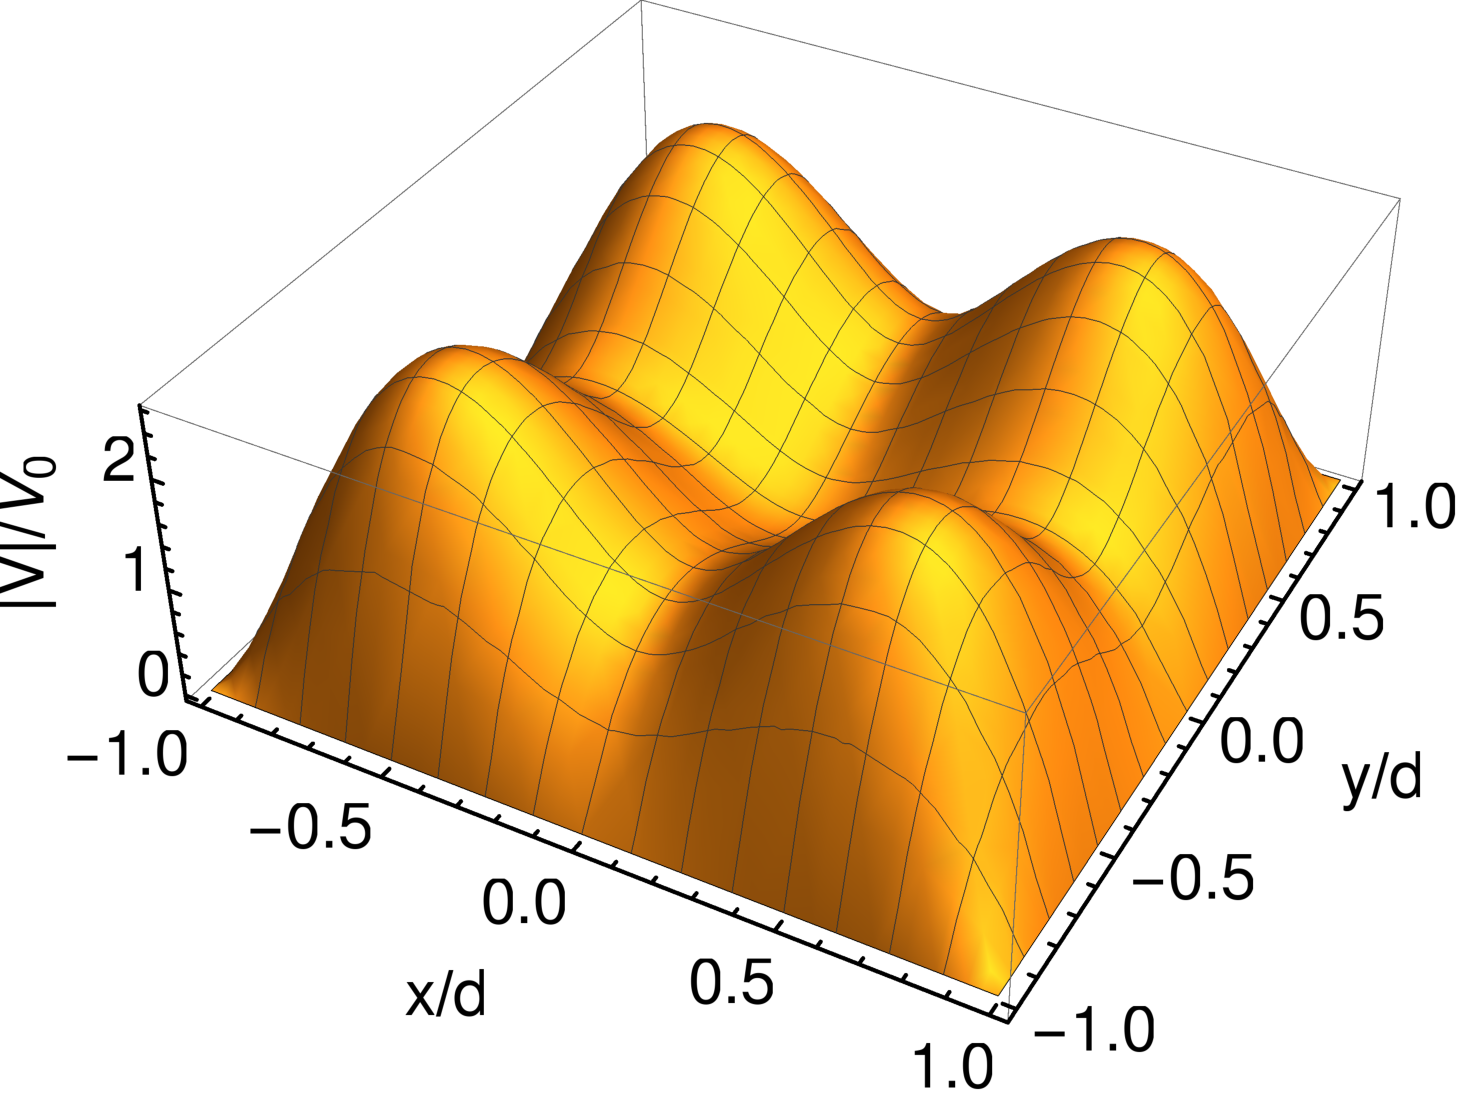
\includegraphics[width = 0.6\columnwidth]{Figures/fig_T_A_pot_abs.pdf}\\
    (b)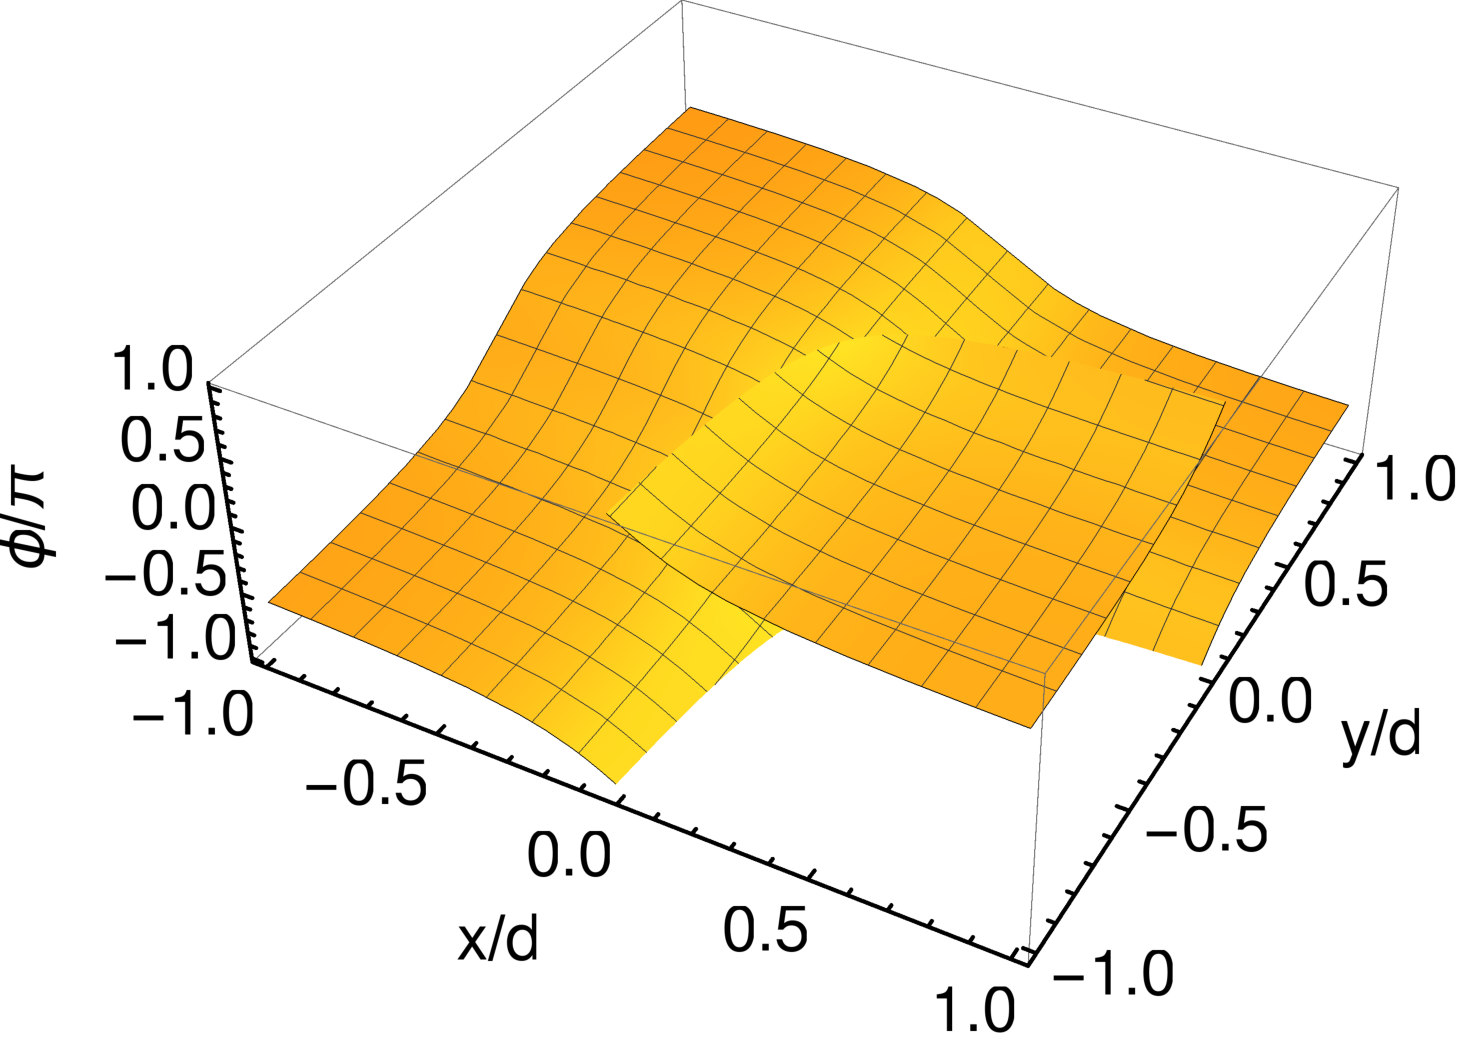
\includegraphics[width = 0.6\columnwidth]{Figures/fig_T_A_pot_arg.pdf}\\
    (c)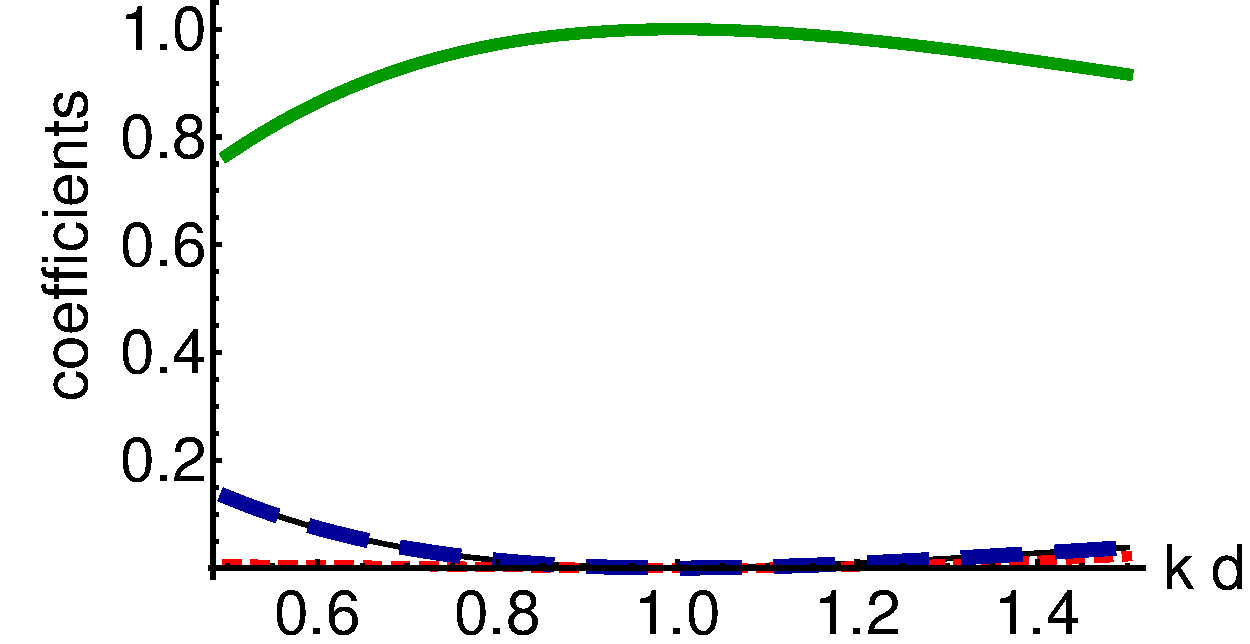
\includegraphics[width = 0.6\columnwidth]{Figures/fig_T_A_prob.pdf}
  \end{center}
  \caption{(Color online) One-way T-filter ($\cal{T/A}$, $\left|T^l\right|=1,T^r=R^l=R^r=0$) with  potential $V(x,y)=|V(x,y)|e^{i\phi(x,y)}$ set
  for $k_0 = 1/d$.
  (a) Absolute value $\left| V(x,y) \right|$;    (b) Argument $\phi(x,y)$;
  (c) Transmission and reflection coefficients:
  $\left| R^l \right|^2$ (black, solid line), $\left| T^l \right|^2$ (green, solid line),
  $\left| R^r \right|^2$ (blue, tick, dashed line), $\left| T^r \right|^2$ (red, dotted line). $V_0 = \hbar^2/(2m d^3)$.\label{fig_device_T_A}}
\end{figure}


%
%
%

\section{Designing potentials for asymmetric devices\label{examples}}

\begin{figure}
  \begin{center}
    (a) 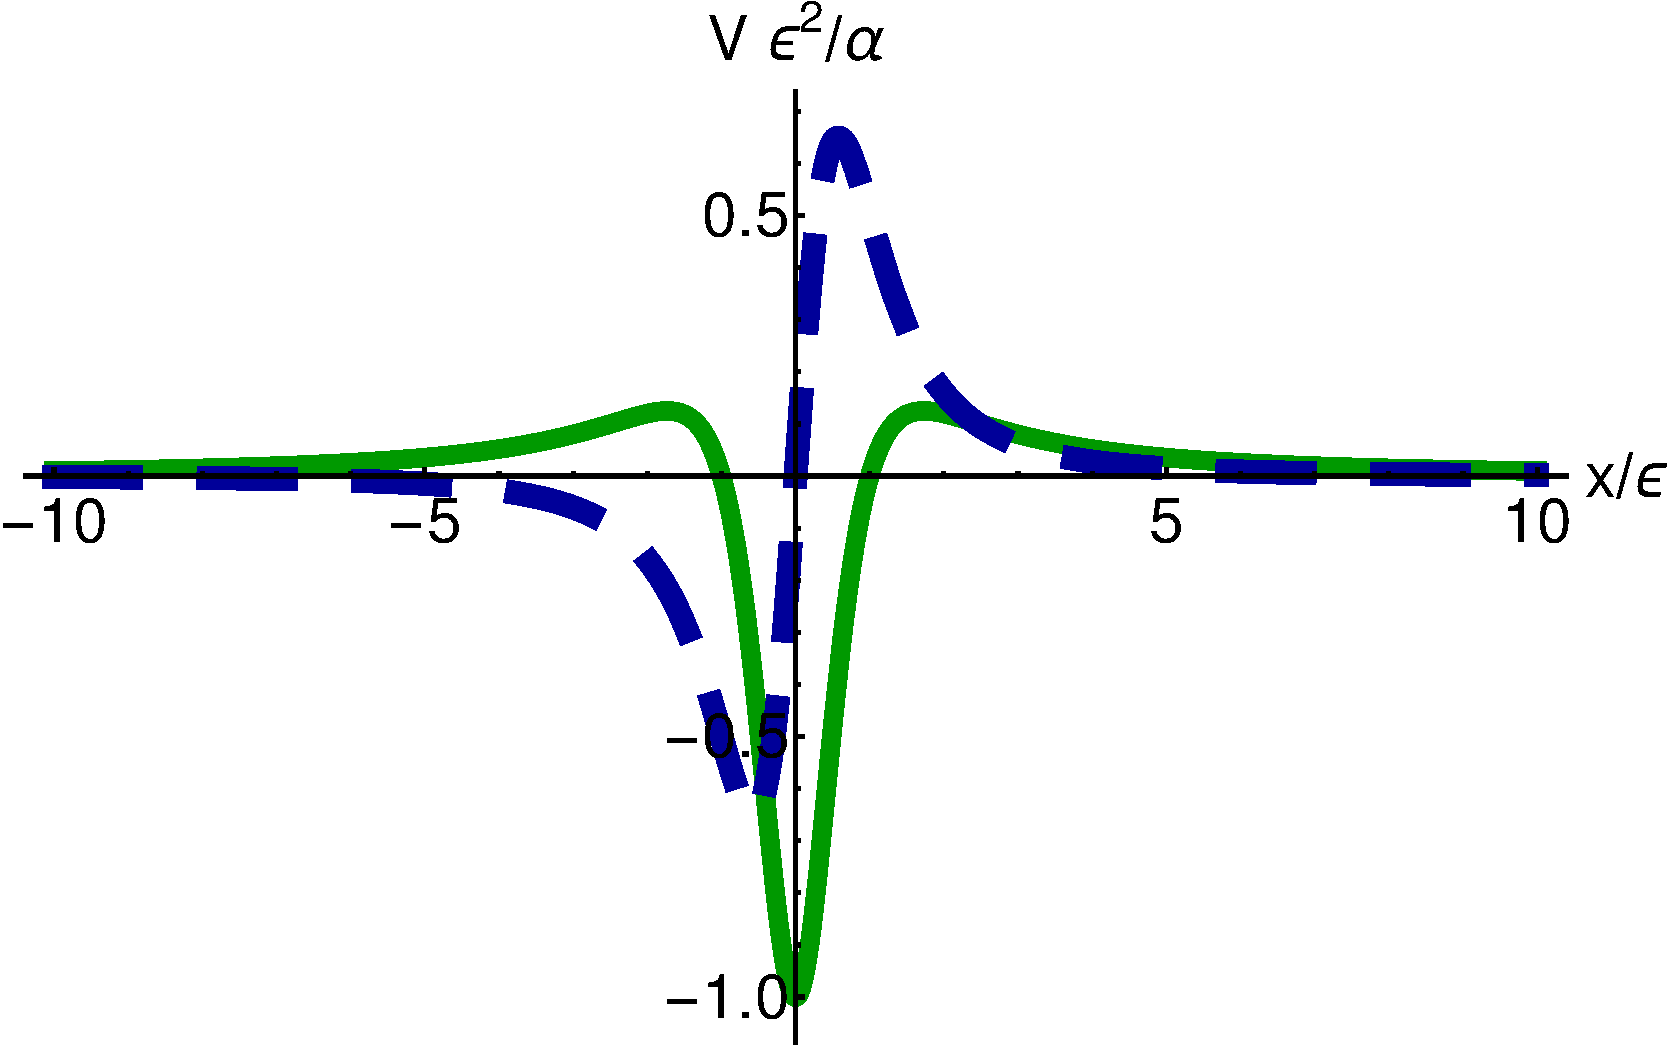
\includegraphics[width = 0.6\columnwidth]{Figures/fig_TR_T_local_pot.pdf}\\
    (b) 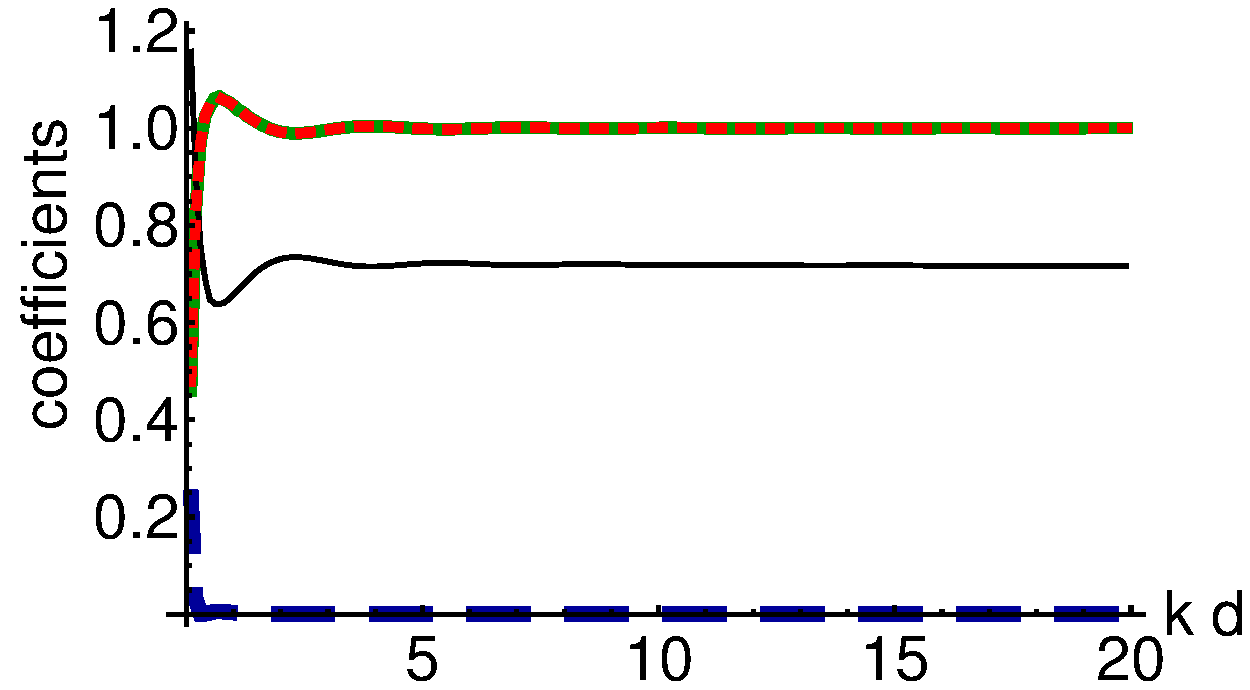
\includegraphics[width = 0.6\columnwidth]{Figures/fig_TR_T_local_prob_1.pdf}\\
    (c) 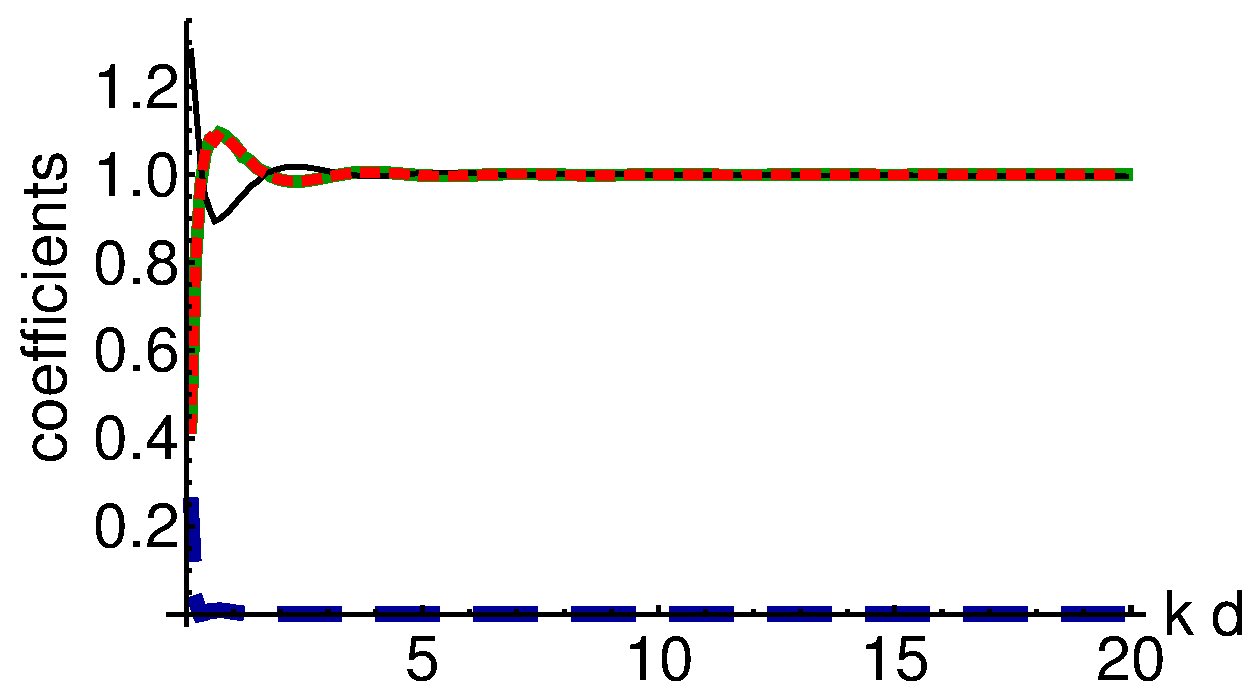
\includegraphics[width = 0.6\columnwidth]{Figures/fig_TR_T_local_prob_2.pdf}
  \end{center}
  \caption{\label{fig_reflector}(Color online) Transparent 1-way reflector with a local PT potential:
  (a) Approximation of the potential (\ref{num}), real part (green solid line), imaginary part (blue dashed line).
  (b,c) Transmission and reflection coefficients versus momentum $k d$;
  left incidence: $\left| R^l \right|^2$ (black, solid line), $\left| T^l \right|^2$ (green, solid line);
  right incidence: $\left| R^r \right|^2$ (blue, tick, dashed line), $\left| T^r \right|^2$ (red, dotted line, coincides with green, solid line).
  $\epsilon/d = 10^{-4}$.
  (b) $\alpha= 1.0 \hbar^2/(4\pi m)$ (c) $\alpha = 1.225 \hbar^2/(4\pi m)$
  (the black, solid line coincides here mostly with the red, dotted and green, solid lines).
  \label{fig_TR_T_local}}
\end{figure}


We will show  how to design non-local potentials
leading to the asymmetric devices.
For simplicity we look for  non-local potentials $V(x,y)$ with local support
that vanish  for $|x| >d$ and $|y| >d$.

Inverse scattering proceeds similarly to \cite{Palao1998},
by imposing an ansatz
for the wavefunctions and the potential
in the stationary Schr\"odinger equation
%
\begin{eqnarray}
  \frac{\hbar^2k^2}{2m} \psi (x) = - \frac{\hbar^2}{2m} \frac{d^2}{dx^2} \psi (x)
  +\!\!\int_{-d}^d \!dy V(x, y) \psi(y).
  \label{Schroedinger}
\end{eqnarray}
%
The free parameters are fixed making use of the boundary conditions.
The form of the wavefunction incident from the left is
$\psi_l(x) = e^{i k x} + R^l e^{-i k x}$ for $x < -d$ and $\psi_l (x) = T^l e^{i k x}$ for $x > d$,
where  $k=p/\hbar$.
The wavefunction incident from the right is instead
$\psi_r(x) = e^{-ikx} T^r$ for $x < -d$ and $\psi_r (x) = e^{-i k x} + R^r e^{i k x}$ for $x > d$.

Our strategy is to assume  polynomial forms for the two wavefunctions in the interval $|x| < d$,
$\psi_l (x) = \sum_{j=0}^5 c_{l,j} x^j$ and $\psi_r (x) = \sum_{j=0}^5 c_{r,j} x^j$, and also a
polynomial ansatz of finite degree for the potential $V(x,y) = \sum_i \sum_j v_{ij} x^i y^j$.
Inserting these ansatzes in eq. (\ref{Schroedinger}) and from the conditions that $\psi_{l,r}$
and their derivatives must be continuous, all coefficients $c_{l,j}\,,c_{r,j}$ and $v_{ij}$ can be determined.
Symmetry properties of the potential can also be imposed via additional conditions on
the potential coefficients $v_{ij}$. For example we may use this method to obtain a one-way T-filter ($\cal{T/A}$) device (third device in table \ref{table1}) with a nonlocal PT-pseudohermitian potential (symmetry VIII of table \ref{table2}) for a chosen wavevector $k = k_0$. The absolute value and argument of the resulting potential $V(x,y)$ are shown in figs. \ref{fig_device_T_A}(a) and \ref{fig_device_T_A}(b) together with its scattering coefficients as function of the incident wave vector, fig. \ref{fig_device_T_A}(c). As can be seen in fig. \ref{fig_device_T_A}(c) the imposed scattering coefficients are fulfilled exactly for the chosen wavevector. They are also satisfied approximately in a neighborhood of $k_0$. In the  Supplemental Material, Sec. II, we give further details about the construction of this potential and we work out other asymmetric devices of fig. \ref{cases}.
%
% ---------------------------------------- Asymmetric Reflection -----------------------------------
%
%
%
%

%
%%%%%%%%%%%%%%%%%%%%%%%%%%%%%%%%%%%%%%%%%%%%%%

%%%%%%%%%%%%%%%%%%%%%%%%%%%%%%%%%%%%%%%%%%%%%
%

\section{Extending the scattering asymmetry to a broad incident-momentum domain\label{ext}}
%
%
%
%
The inversion technique just described may be generalized
to extend the range of incident momenta for which the potential works by imposing additional
conditions and increasing correspondingly the number of parameters in the wavefunction ansatz,
for example we may impose that the derivatives of the  amplitudes,  in one or more orders,  vanish at $k_0$,
or  0/1 values for the coefficients not only at  $k_0$ but at a series of grid points $k_1$, $k_2$, ... $k_N$,
as in \cite{Brouard1994,Palao1998a,Palao1998,Muga2004}.

Here we put forward instead a method that provides a very broad working-window domain.
While we make formally use of the Born approximation, the exact numerical
computations demonstrate the robustness and accuracy of the approach to achieve that objective by
making use of an adjustable parameter in the potential. The very special role of the Born approximation in inverse problems has been
discussed and demonstrated in \cite{Snieder1990,Mostafazadeh2014,Horsley2015}.
Specifically we study a transparent one-way reflector ${\cal{TR/T}}$.
Our aim is now to find a local PT-symmetric potential such that asymmetric reflection results,
$T^l = T^r = 1, R^r = 0, |R^l|=1$ for a broad range of incident momenta. A similar goal
was pursued in \cite{Longhi2014} making use of a supersymmetric transformation,
without imposing $|R^l|=1$.

In the Born approximation and for a local potential $V(x)$, the reflection amplitudes take the simple form
%
\begin{eqnarray}
  R^l=-\frac{2\pi i m}{p}\langle -p|V|p\rangle,
  \;
  R^r=-\frac{2\pi i m}{p}\langle p|V|-p\rangle.
\end{eqnarray}
%
Defining the Fourier transform
%
\begin{eqnarray}
  \widetilde V (k) = \frac{1}{\sqrt{2\pi}} \int_{-\infty}^\infty dx \, V(x) e^{-i k x}
\end{eqnarray}
%
we get for $k=p/\hbar>0$:
%
\begin{eqnarray}
  R^l=-\frac{\sqrt{2\pi} i m}{k \hbar^2} \widetilde V (-2k),
  \;
  R^r=-\frac{\sqrt{2\pi} i m}{k\hbar^2} \widetilde V (2 k).
\end{eqnarray}
%
Assuming that the potential is local and PT-symmetrical, we calculate the transition coefficient
from them using generalized unitarity as
$|T|^2=1-{R^r}^*R^l$.

To build a ${\cal{TR/T}}$ device we demand:
$\widetilde V(k) = \sqrt{2\pi} \alpha k$ ($k < 0$) and $\widetilde V(k) = 0$ ($k \ge 0$).
By inverse Fourier transformation, this implies
%
\begin{eqnarray}
  V(x) &=&
  %-\alpha \frac{\partial}{\partial x} \left[P \frac{1}{x} + i \pi \delta(x) \right]
  %\nonumber\\
  %&=&
  -\alpha \frac{\partial}{\partial x} \lim_{\epsilon\to 0} \frac{1}{x - i \epsilon}
  = \alpha \lim_{\epsilon\to 0} \frac{1}{(x - i \epsilon)^2}
  \nonumber\\
  %&=& \alpha \lim_{\epsilon\to 0} \frac{(x + i \epsilon)^2}{(x^2 + \epsilon^2)^2}\\
  &=& \alpha \lim_{\epsilon\to 0} \left[\frac{x^2 - \epsilon^2}{(x^2 + \epsilon^2)^2} + i
  \frac{2 x\epsilon}{(x^2 + \epsilon^2)^2}\right],
  \label{num}
\end{eqnarray}
%
which is indeed a local, $PT$-symmetric potential for $\alpha$ real.
$\alpha$ is directly related to the reflection coefficient, within the Born approximation,
$R^l = 4 \pi i m \alpha/\hbar^2$. As the Born approximation may differ from exact results
we shall keep $\alpha$ as an adjustable parameter
in the following.

In a possible physical implementation, the potential in eq. (\ref{num}) will
be approximated by keeping a small finite $\epsilon>0$, see fig. \ref{fig_TR_T_local}(a).
%\begin{eqnarray}
%V(x) = \alpha \left[\frac{x^2 - \epsilon^2}{(x^2 + \epsilon^2)^2} + i
%\frac{2 x\epsilon}{(x^2 + \epsilon^2)^2}\right],
%\end{eqnarray}
%with a finite, small $\epsilon>0$.
Then, its Fourier transform is
$\widetilde V(k) = \sqrt{2\pi} \alpha k e^{\epsilon k}$ ($k < 0$) and $\widetilde V(k)=0$ ($k \ge 0$).
In figs. \ref{fig_TR_T_local}(b) and (c), the resulting coefficients for $\epsilon/d=10^{-4}$ and  two different values
of $\alpha$ are shown.  These figures have been calculated by
numerically solving the Schr\"odinger equation exactly.
% and demonstrate that
%$\alpha$ can indeed  be adjusted so that $\left| R^l \right|^2 \approx 1$.
Remarkably, the Born approximation contains all the information required to build the required potential shape
up to a global factor.  Such a prominent role of the Born approximation in inverse problems has been noted
in different applications \cite{Snieder1990,Mostafazadeh2014,Horsley2015}. For a range of $\alpha$, the potential gives $|R^r|\approx 0$, a nearly constant $|R^l|^2$, and
$|T^r|= |T^l|\approx1$  in a broad $k$-domain, see fig. \ref{fig_TR_T_local}(b). Adjusting  the value of $\alpha$, fig. \ref{fig_TR_T_local}(c),
sets $|R^l|\approx 1$ as desired.
%
%Remarkably, except for very low $k$,
%the potential is reflectionless from the right
%and provides full transmission independently of $\alpha$. As well, $|R^2|^2$ stays constant with respect to $k$ for different $\alpha$,
%so that that up to the adjustable parameter the Born approximation provides in fact the required potential shape, a surprising
%in inverse problems \cite{Snieder1990,Mostafazadeh2014,Horsley2015}.
%Figure \ref{fig_TR_T_local}(c) demonstrates that $\alpha$ can indeed be adjusted so that the  potential works
%as intended, i.e., as a transparent one-way reflector,  for a very broad range of $k$ values.

%
%
%
%
%
\section{Discussion}
%
%
Scattering asymmetries are necessary to develop technologically relevant devices such
as one-way mirrors, filters and  barriers, invisibility cloaks, diodes, or Maxwell demons.
So far much effort has been devoted to build and apply local  PT-symmetric potentials but the possible scattering asymmetries with them are
quite limited.
%This paper shows that to realize all possible devices it is necessary to go beyond local PT-potentials to
%ealize different asymmetric devices.
We find that six  device types with asymmetric scattering are possible
when imposing $0$ or $1$ scattering coefficients.
PT-symmetry can only realize one of them, but this symmetry  is just one among eight possible symmetries of complex non-local potentials.
The eight symmetries arise from the discovery that Klein's four-group
$\{1, \Pi, \Theta, \Theta\Pi\}$, combined with two possible relations among the Hamiltonian, its adjoint,
and the symmetry operators of the group, eqs. (1) and (2),
produce all possible  equalities among potential matrix elements after complex conjugation, coordinate inversion, the identity, and transposition.
In other words, to have all possible such equalities, the conventional definition of a symmetry $A$ in terms of its commutation with the Hamiltonian $H$ is not enough, and $A$-pseudohermiticity must be considered as well on the same footing.
Extending the concept of what a �symmetry� is for complex, non-local potentials is
a fundamental, far-reaching step of this work.
This group theoretical analysis and classification is not only esthetically pleasing, but also of practical importance, as it reveals
the underlying structure and span of the possibilities available in principle to manipulate the asymmetrical response of a potential
for a structureless particle.

%This paper brings to the fore the essential role of eight generalized symmetries to determine the
%transmission and reflection asymmetries by complex, and possibly nonlocal potentials.
%These symmetries are classified with the aid of the relations between
%unitary or antiunitary operators $1, \Pi, \Theta, \Theta\Pi$, which form Klein's 4-group,
%and $H$ or its adjoint.
%generically $A$, forming Klein's 4-group
%and correspond to $A$ either commuting with
%the Hamiltonian $H$, or intertwining
%$H$ and $H^\dagger$ as $AH=H^\dagger A$.
%The symmetries set equalities among the scattering
%amplitudes which, complemented by generalized unitarity relations, tell us which symmetries allow or disallow
%a certain device with asymmetric scattering. Simplifying the analysis by imposing $0$ or $1$ scattering coefficients,
%six possible device types exist.
%We provide examples of potentials
We provide potentials for the different asymmetric  devices including an example that works
in a broad domain of incident momenta.
%
Although the present theory is for the scattering of quantum particles, the analogies between quantum physics and optics suggest to extend the concepts and results for optical asymmetric devices.

Interesting questions left for future work are  the inclusion of other mechanisms for transmission and reflection asymmetries (for example
nonlinearities \cite{Xu2014,Konotop2016}, and  time dependent potentials \cite{Yu2009,Longhi2017}),
or a full discussion of the phases of the scattering amplitudes
in addition to the moduli emphasized here. In this paper the properties of the scattering amplitudes have been worked out assuming that the operator $A$ in the symmetry relations in eqs. (\ref{symm}) and (\ref{pseudo}) is a unitary/antiunitary operator in Klein's group.
We may generalize the study to include more general operators, possibly including differential operators, as was done in \cite{Konotop2017} for phase transitions of optical potentials, or the operator that swaps internal states or waveguides \cite{Kartashov2014,Zezyulin2017}.

We shall also examine in a complementary paper the physical realization of complex nonlocal effective potentials.
In a quantum optics scenario, simple examples were provided in \cite{Ruschhaupt2004a} based on applying the partitioning technique \cite{Feshbach1958,Feshbach1962}
to the scattering of a particle with internal structure. The experimental realization
of all new symmetries and devices may be challenging, e.g. to engineer the nonlocality in optics,
but there is much to gain.  We may expect progress similar to
the successful evolution from theory to actual devices in the sequence from the first mathematical
models of PT-symmetric potentials \cite{Bender1998}, to the proposal of an optical realization \cite{Ruschhaupt2005}, and to the actual experiments \cite{Guo2009},  even if considerable time lapses were needed between the three steps.
%
